\documentclass{article}
\usepackage{textcomp}
\usepackage{float}

% Basic packages
\usepackage[utf8]{inputenc}
\usepackage[T1]{fontenc}
\usepackage{lmodern}
\usepackage[margin=2.5cm]{geometry}
\usepackage{amsmath,amssymb}
\usepackage{hyperref}
\usepackage{graphicx}
\usepackage{booktabs}
\usepackage{enumitem}
\usepackage{natbib}
\usepackage{xcolor}
\usepackage{float}
\usepackage{doi}
\usepackage{url}
\usepackage[font=small,labelfont=bf]{caption}
\captionsetup[table]{labelsep=quad}
\usepackage{ragged2e}
\usepackage{array}
\newcolumntype{L}[1]{>{\RaggedRight\arraybackslash}p{#1}}
\usepackage{enumitem}
\setlist[itemize,1]{label=---}
% Define PDL macro
\newcommand{\PDL}{\mathrm{PDL}}
\usepackage{tikz}
\usetikzlibrary{positioning}
\usepackage{longtable}
\usetikzlibrary{positioning}
\usetikzlibrary{backgrounds}
\usepackage{booktabs} % tu l'as déjà, gardons-le

\hypersetup{
  colorlinks=true,
  linkcolor=blue,
  citecolor=blue,
  urlcolor=blue
}

\title{Projective Dynamic Logo (PDL)\\
Global Mapping of Structures, Results, and Open Problems}
\author{C. Laubscher}
\date{\today}

\begin{document}

\setcounter{tocdepth}{1}

\maketitle

\begin{abstract}
This document presents a comprehensive and systematic exposition of the Projective Dynamic Logo (PDL) framework at a global level. It synthesizes the existing body of work into a unified, coherently articulated theoretical architecture, elucidates the logical dependencies among axioms, formal constructions, and their associated physical interpretations, and classifies the resulting propositions according to their epistemic status. Specifically, it distinguishes rigorously established structural theorems from tightly circumscribed conjectural hypotheses, as well as from model components whose parameters are inferred or constrained through empirical calibration.
\end{abstract}
\tableofcontents

\section{Purpose and Scope}
\label{sec:purpose_scope}

\subsection{Aim of this mapping}
\label{subsec:aim}

The purpose of this mapping document is to provide a systematic and comprehensive overview of the Projective Dynamic Logo (PDL) programme. Rather than presenting novel technical results, it synthesises and organises the existing body of work into a coherent conceptual framework, thereby elucidating the interrelations among axioms, constructions, and physical interpretations, as well as their respective epistemic status \citep{PDL_position,PDL_intro}. More specifically, this document pursues four principal objectives: (i) to make explicit the logical dependencies among the core components of PDL (relational axioms, minimal $4$--$6$ block, proton architecture, constants, dynamics, leakage mechanisms, and emergent metric structure); (ii) to classify existing results into rigorously established structural theorems, tightly constrained conjectures, and empirically calibrated components; (iii) to function as a navigational tool for the PDL corpus by means of concise summaries and systematic cross-references; and (iv) to delineate a research agenda of open problems and prospective directions for further investigation \citep{PDL_position}.

\subsection{Position within the PDL corpus}
\label{subsec:position_corpus}

Within the broader PDL corpus, the present mapping document is to be interpreted as a meta-level contribution. The principal PDL/LDP article (D1) develops the full axiomatic framework, including the derivation of the $4$–$6$ structural pattern, the specification of the proton architecture, and a reformulation of several physical constants, and further provides an initial treatment of gravitation and cosmology \citep{PDL_Main_2026}. The introductory note (D2) offers a high-level conceptual overview together with a concise synopsis of the main structural features and numerical correspondences \citep{PDL_intro}. The position paper (D3) examines the current status of the framework, its epistemic stratification, and the principal unresolved questions, with particular attention to its interface with the Theory of Objectivity \citep{PDL_position}. In contrast, the present mapping does not supersede any of these texts; instead, it systematises their content by supplying an explicit dependency diagram, a unified classification of results, and a cross-referenced index of documents and thematic domains.

Beyond these three foundational texts, several more recent manuscripts elaborate specific components of the programme in greater technical detail. In particular, the logical core and the necessity of the $(4,6)$ block are investigated in a dedicated study on minimal stationary closures~\citep{Minimal_Stationary_Closures_2026}; the combinatorial selection mechanisms and local uniqueness properties of the proton architecture are analysed in a more refined manner~\citep{Proton_Local_Uniqueness_2026,Combinatorial_Proton_v2_2026}; and the leakage mechanism, together with the exponent $18$, is re-examined in a more systematic fashion~\citep{Coherence_Leakage_18_2026,Exponent_18_PDL_2026}. Furthermore, a philosophically oriented reflection on existence as pulsating closure articulates the ontological commitments of PDL and its treatment of boundaries, active surfaces, and transcendence~\citep{ExistencePulsatingClosure2026}, while a recent investigation of discrete cavity modes and the logical density of states establishes that a purely relational PDL cavity can support low-leakage periodic excitations with an emergent three-dimensional $\rho(\nu)\propto \nu^2$ density-of-states profile~\citep{PDLCavityModes2026}.

\subsection{Intended audience}
\label{subsec:intended_audience}

The primary target audience for this exposition comprises researchers in foundational physics, mathematical physics, quantum foundations, and related conceptual research programmes, including the Theory of Objectivity. It is intended for readers with a high level of proficiency in abstract structural reasoning and discrete mathematical formalisms, who seek a succinct yet systematic account of the current claims of PDL, the manner in which its constituent components integrate into a coherent framework, and the identification of the most salient open problems \citep{PDL_intro,PDL_TO_dialogue,PDL_position}. It is not conceived as a popular-level introduction, nor as a replacement for the detailed technical derivations provided in the primary PDL source manuscripts.

\section{Overview of the PDL Programme}
\label{sec:overview}

\subsection{Core question and methodological stance}
\label{subsec:core_question}

The PDL programme is organised around a single central research question: \emph{What are the minimal logical conditions under which an entity can exist in a temporally persistent manner, once all metric notions such as space, time, and energy have been suspended}? \citep{PDL_Main_2026,PDL_intro}

In contrast to approaches that presuppose a pre-given spacetime manifold, a fixed set of elementary particles, or externally imposed dynamical laws, PDL adopts a more fundamental, pre-metric standpoint. It assumes solely that existence must appear as a reproducible distinction—a difference that can be instantiated repeatedly in a way that is logically self-sufficient, independent of any unspecified background structure, and capable of being stably maintained without collapsing into an undifferentiated null state.
\citep{PDL_Main_2026,PDL_position}.

Within this theoretical framework, reality is represented as a network of minimal logical closures defined over finite signed graphs. The vertices correspond to informational entities, while the edges encode binary relations of agreement or disagreement. The dynamical evolution of the resulting configurations is determined by a coherence-optimization principle, rather than by externally imposed field equations. Space, time, and other familiar physical observables are not posited as primitive entities but are instead regarded as potentially emergent structures, to be systematically reconstructed from the coherence properties exhibited by these closures.
\citep{PDL_Main_2026,PDL_intro}.

Methodologically, this gives rise to a two-stage procedure. In the first stage, one formulates purely relational axioms that specify the logical conditions for persistent existence—namely, minimal binary pulsation, triangular coherence, minimal completeness, and logical optimisation. In the second stage, one investigates which discrete structures are \emph{necessarily} instantiated under these axioms and to what extent they can be coherently identified with known physical entities, such as the electron, the proton, and various dimensionless constants. The present mapping document is devoted to clarifying the manner in which this strategy is implemented across the existing PDL corpus.
\citep{PDL_position}.

\subsection{List of main PDL documents}
\label{subsec:documents}

Table~\ref{tab:documents} presents a synoptic overview of the principal documents constituting the current PDL corpus, specifying their predominant thematic orientation and explicating their respective roles within the overarching programme architecture.

\setlength{\LTpre}{18pt}
\setlength{\LTpost}{0pt}

\begin{longtable}{@{}llL{4cm}p{9.5cm}@{}}
\caption{Main PDL documents and their roles within the programme.}
\label{tab:documents}\\
\toprule
Label & Year & Document & Focus / Role \\
\midrule
\endfirsthead

\toprule
Label & Year & Document & Focus / Role \\
\midrule
\endhead

D1 & 2026 & \textit{The Emergence of Physical Reality within the Framework of the Projective Dynamic Logo (PDL)} &
Principal technical article: formulation of relational axioms on signed graphs; derivation of the minimal $(4,6)$ structural block; development of a hierarchical proton architecture; reinterpretation of $\hbar$, $\alpha$, $k_B$, and an effective gravitational coupling constant as coherence ratios; and preliminary construction of an emergent metric and cosmological framework. \citep{PDL_Main_2026} \\[0.5em]

D2 & 2026 & \textit{Introduction to the Projective Dynamic Logo (PDL)} &
High-level exposition of the PDL framework, including conceptual motivation, outline of the axiomatic system, presentation of the $(4,6)$ structure, analysis of the proton integers $(24,28,930,10087,11017)$, and a unified treatment of fundamental constants aimed at readers in quantum foundations and mathematical physics. \citep{PDL_intro} \\[0.5em]

D3 & 2026 & \textit{Projective Dynamic Logo as a Foundational Research Programme: Current Status, Open Problems, and Interface with the Theory of Objectivity} &
Position paper: synthesises the current state of the programme, delineates structurally robust results from conjectural or calibrated components, and formulates open problems (including uniqueness of the $(4,6)$ configuration, rigidity of the proton architecture, derivation of the leakage parameter, and dynamical extensions), with emphasis on the interface with the Theory of Objectivity. \citep{PDL_position,PDL_TO_dialogue} \\[0.5em]

D4 & 2026 & \textit{On the Combinatorial Selection of the Proton Architecture in PDL: Axiomatic Constraints, Integer Structures, and a Uniqueness Conjecture (v2)} &
Updated analysis of the proton structural configuration: formulation of integer-valued constraints, specification of an optimisation functional, and justification of the parameter tuple $(24,28,930,10087,11017)$ in its v2 form, together with a critical discussion of potential alternative architectural configurations. \citep{Combinatorial_Proton_v2_2026} \\[0.5em]

D5 & 2026 & \textit{A Structural Derivation of the Fine-Structure Constant from the Projective Dynamic Logo (PDL) (v2)} &
Closed-form expression for $\alpha^{-1}$ as a function of the proton–electron mass ratio, the valence content $r_{\mathrm{val}}=930$, and the golden ratio, achieving a relative accuracy of $\mathcal{O}(10^{-4})$ without continuous fit parameters; v2 incorporates refinements after the TO dialogue. \citep{Alpha_PDL_v2_2026} \\[0.5em]

D6 & 2026 & \textit{Relational Emergence of Born's Rule and a Golden-Ratio Active Surface in PDL (v2)} &
Derivation of Born's rule for spin-$\tfrac{1}{2}$ systems and of the fine-structure constant from finite active surfaces in signed graphs; refinement of the rôle of the golden ratio in the proton core–surface partition and its connection to $\alpha$; v2 incorporates structural clarifications. \citep{Born_Golden_v2_2026,Golden_Ratio_Sketch_2026} \\[0.5em]

D7 & 2026 & \textit{From Discrete Coherence Flux to Effective Fields: A Structured Programme within the PDL Framework} &
Development of discrete Gauss- and Faraday-like relations from mixed-triangle coherence fluxes in PDL, derivation of $1/r^2$ Coulomb profiles from shell-counting arguments, and outline of how Schr\"odinger-type dynamics can emerge from discrete coherence flux. \citep{Effective_Fields_PDL_2026} \\[0.5em]

D8 & 2026 & \textit{A Minimal Relational Sketch for the Emergence of the Golden Ratio in PDL} &
Conceptual sketch showing how a self-similar core–surface partition within the proton architecture leads to the selection of the golden ratio and constrains the effective active surface associated with $\alpha$ and surface coherence. \citep{Golden_Ratio_Sketch_2026} \\[0.5em]

D9 & 2026 & \textit{Hierarchical Filtering of Coherence Leakage and Justification of the Exponent 18 in PDL} &
Initial formulation of the leakage mechanism and of the exponent $18$ as the total number of hierarchical coherence filters linking proton-level leakage to macroscopic effective couplings; provides the original list of filters and qualitative arguments for their minimality. \citep{Exponent_18_PDL_2026} \\[0.5em]

D10 & 2026 & \textit{Logical Leakage as Self-Maintained Probability: A Topological Reformulation in the Projective Dynamic Logo Framework} &
Development of a coexistence topology and a coherence-cost pseudo-metric, reinterpreting logical leakage as an intrinsic probability of non-closure, and exploring correspondences with quantum probabilities, gravitation, and thermodynamics. \citep{Topological_Reformulation_PDL_2026} \\[0.5em]

D11 & 2026 & \textit{Compatibility of the Schr\"odinger Framework with the Projective Dynamic Logo (PDL) (v2)} &
Consistency assessment: implementation of the PDL-derived fine-structure constant and proton parameters into the nonrelativistic hydrogenic Schr\"odinger equation; verification of spectral concordance within stated accuracy; v2 updates the analysis and numerical checks. \citep{Schrodinger_PDL_v2_2026} \\[0.5em]

D12 & 2026 & \textit{Towards a Schr\"odinger--Type Dynamics from the Projective Dynamic Logo (PDL): A Relational Sketch Linking Coherence Cycles, Active Surfaces, and Effective Potentials (v2)} &
Investigation of how Schr\"odinger-like dynamical equations might emerge from intrinsically defined discrete graph evolution (Laplacians and flux balance) rather than being postulated; v2 refines the relational sketch and its consistency conditions. \citep{Schrodinger_Sketch_v2_2026} \\[0.5em]

D13 & 2026 & \textit{A Modal Dialogue between the Projective Dynamic Logo (PDL) and the Theory of Objectivity (TO)} &
Comparative study of PDL relational axioms and TO's Seven Absolute Truths; clarification of modal and ontological commitments of PDL and formal treatment of multi-observer perspectives and boundary conditions. \citep{PDL_TO_dialogue} \\[0.5em]

D14 & 2026 & \textit{Towards an Einstein--Dirac Unification from the Projective Dynamic Logo Framework} &
Extension of PDL towards a unified treatment of Einstein- and Dirac-type structures: association of Dirac spinors with $(4,6)$ electron closures, coupling to the emergent coherence-cost metric, and preliminary consistency checks based on hydrogenic limits and redshift-type scenarios. \citep{Einstein_Dirac_PDL_2026} \\[0.5em]

D15 & 2026 & \textit{Minimal Stationary Closures in the Projective Dynamic Logo Framework: Necessity of the (4,6) Block} &
Technical analysis of the logical core: reformulation of the four PDL axioms directly on finite signed graphs; introduction of a precise notion of minimal stationary closure; proof that no such closure exists for graphs with at most three vertices and that the complete signed graph on four vertices and six edges realises the first admissible elementary stationary closure, with minimality and quasi-uniqueness properties. \citep{Minimal_Stationary_Closures_2026} \\[0.5em]

D16 & 2026 & \textit{On the Combinatorial Selection and Local Uniqueness of the Proton Architecture in the PDL Framework} &
Refined combinatorial treatment of the proton architecture: definition of admissible proton configurations under structural and phenomenological constraints, introduction of a selection functional $S$, verification that the tuple $(24,28,930,10087,11017)$ is admissible and achieves a high selection score, and formulation of an explicit local uniqueness conjecture and search programme. \citep{Proton_Local_Uniqueness_2026,Combinatorial_Proton_v2_2026} \\[0.5em]

D17 & 2026 & \textit{Coherence Leakage, Hierarchical Filtering, and the Exponent 18 in the Projective Dynamic Logo Framework} &
Refined treatment of coherence leakage and the exponent $18$: definition of the minimal closure defect $\varepsilon$ on a class of admissible proton graphs, interpretation of $\varepsilon$ as an intrinsic coherence leakage parameter, organisation of the eighteen coherence filters into three hierarchical blocks, and formulation of an effective coupling ansatz $G_{\mathrm{eff}}^{\PDL}=C\,\varepsilon^{n}$ together with qualitative constraints. \citep{Coherence_Leakage_18_2026,Topological_Reformulation_PDL_2026,Effective_Fields_PDL_2026} \\[0.5em]

D18 &
2026 &
\emph{Existence as Pulsating Closure: An Ontological Meditation on the PDL Framework.} & 
Philosophically oriented analysis of PDL as a proposal about persistent existence on finite signed graphs; clarifies the passage from nothingness to minimal pulsating closure, the role of boundaries, active surfaces, and coherence leakage as disciplined notions of transcendence, the coexistence topology and multi-observer stabilisation, and the resonance of the closure/leakage picture with aspects of human experience, while remaining anchored in the technical PDL corpus~\citep{ExistencePulsatingClosure2026}.\\[0.4em]

D19 &
2026 &
\emph{Discrete Cavity Modes and Logical Density of States in the PDL Framework.}
 & Construction of a three-dimensional PDL cavity as a finite signed graph; definition of a photon-like logical excitation governed by a local update rule indexed by $(n_x,n_y,n_z)$; numerical identification of low-leakage periodic modes with minimal period $N(n_x,n_y,n_z)=4(n_x+n_y+n_z)$ for a broad family; and derivation of an effective logical density of states scaling $\rho(\nu)\propto \nu^2$ in three dimensions, in direct analogy with continuum cavity mode counting~\citep{PDLCavityModes2026}.\\[0.4em]

D20 & 2026 &
\textit{Universal Coherence Leakage: Bridging Gravitational and Fine-Structure Constants through Discrete Relational Closures} &
Introduction of a primary proton-level coherence-leakage parameter $\varepsilon_G$ on the
$(r_{\mathrm{val}},R_{\mathrm{sea}})=(930,10087)$ partition; inversion of the exponent-18 hierarchical filtering
$\alpha_G = G m_p^2 / (\hbar c) \simeq \varepsilon_G^{18}$ to obtain $\varepsilon_G \approx 0.0073891$; and
identification of a geometric bridge to the electromagnetic sector via an electromagnetic valence surplus
$\Delta r_{\mathrm{val}} \approx 0.0497507$ satisfying $\Delta r_{\mathrm{val}} \approx 3\,\varphi^2 \varepsilon_G$, thereby
locking the gravitational coupling and the fine-structure constant to a single combinatorial defect in the
proton architecture.\citep{Universal_Coherence_Leakage_2026} \\\\[0.5em]

\bottomrule
\end{longtable}

\subsection*{Reading guide}

For readers engaging with PDL for the first time, the following minimal reading pathways are recommended. To acquire a foundational understanding of the logical underpinnings of the programme—encompassing its axiomatic architecture, the minimal $4$–$6$ structure, and the formal representations of the electron and proton—priority should be assigned to Sections~\ref{sec:logical_core}, \ref{sec:four_six_electron}, and \ref{sec:proton_architecture}. For an analysis of the reinterpretation of constants as coherence ratios and the associated emergence of gravitation and metric structure, Sections~\ref{sec:constants} and \ref{sec:topology_metric} should be consulted. A succinct overview of the current status of the theory, distinguishing structurally established results from conjectural or calibrated components, is provided by the global result map in Section~\ref{sec:global_map}, and in particular by Table~\ref{tab:status}. Finally, Section~\ref{sec:roadmap} presents a synthesis of the principal open problems and delineates prospective directions for future research.

\section{Logical Core: Axioms and Minimal Structures}
\label{sec:logical_core}

\subsection{Relational axioms on signed graphs}
\label{subsec:axioms}

In PDL, a logical configuration is formalised as a finite signed graph \(G = (V, E)\), where the vertices \(V\) denote informational entities and the edges \(E\) are assigned signs \(s_{ij} \in \{+1, -1\}\) that encode pairwise relations of agreement or disagreement \citep{PDL_Main_2026,PDL_intro}. On this discrete structural substrate, four relational axioms are postulated:

\begin{itemize}[leftmargin=1.5em]
  \item \textbf{Minimal binary pulsation:} Existence is instantiated as a repeatable alternation between two discrete states that does not presuppose any underlying temporal metric. Formally, the discrete dynamical system defined on the space of sign configurations is required to admit at least one logical 2-cycle.

  \item \textbf{Triangular coherence:} Closed cycles of length three (triangles) are posited as elementary closure motifs. Each violated triangle—either due to the absence of a required edge or to the failure of a coherence condition on the product of signs—contributes a penalty term to a stability functional.

  \item \textbf{Minimal completeness:} Elementary stationary structures must be both closed and logically autonomous: all referential dependencies necessary to maintain the constitutive distinction are required to remain internal to the structure, without appeal to any external background or environment.

  \item \textbf{Logical optimisation:} Among all admissible configurations, dynamically stable configurations are selected as those that maximise a functional jointly favouring low violation of triangular coherence, sufficient relational connectivity, and structural minimality, subject to a global closure constraint.
\end{itemize}

Taken together, these axioms formalise the claim that persistent existence is realised as a closed, self-sustaining relational pattern that minimises logical inconsistency (violated triangles) and suppresses superfluous relational redundancy, while retaining sufficient connectivity to continuously propagate the underlying constitutive distinction \citep{PDL_Main_2026,PDL_position}.

\subsection{Closures and coherence measures}
\label{subsec:closures}

Within this framework, a \emph{closure} is defined as a finite signed graph that realises a self-contained regime of coherence under the axioms specified above. For a given configuration \(G = (V, E)\) endowed with a sign assignment \(s\), the fraction of violated triangles is defined as
\[
  \epsilon \;=\; \frac{\text{number of violated triangles in } G}{\binom{|V|}{3}} \, ,
\]
with the convention \(\epsilon = 0\) whenever \(|V| < 3\). A triangle is classified as violated if at least one of its edges is absent, or if the product of the three associated signs fails to satisfy the closure condition prescribed by the triangular coherence axiom \citep{PDL_Main_2026}.

An optimisation functional is subsequently introduced, depending on \(\epsilon\), on a normalised measure of connectivity, and on an indicator of structural minimality. \emph{Elementary stationary structures} are defined as those configurations that (i) fully satisfy closure (i.e., exhibit no violated triangles), (ii) are complete and connected, (iii) display no internal hierarchy among vertices, and (iv) admit a binary pulsation that preserves coherence. These structures are interpreted as minimal logical primitives or fundamental building blocks \citep{PDL_Main_2026,PDL_position}.

\subsection{Emergence of the minimal 4--6 block}
\label{subsec:4_6_block}

A systematic exclusion of inadequate configurations shows that no graph with fewer than four vertices can realise a homogeneous, non-hierarchical closure satisfying the stipulated axioms. For \(n = 1,2\), triangular subgraphs are entirely absent, and for \(n = 3\) a single triangle is insufficient to sustain the requisite network of overlapping coherent cycles needed for the propagation of internal reference. In each of these cases, the resulting structure either fails to achieve closure, violates autonomy, or induces an implicit hierarchy \citep{PDL_Main_2026}.

The simplest configuration not ruled out by these constraints is the complete graph on four vertices with six edges, denoted \(4,6\). For this graph, it is possible to construct a sign assignment such that all triangular subgraphs are coherent (\(\epsilon = 0\)), the union of coherent triangles forms a single connected component, all vertices are structurally equivalent, and a global sign inversion realises a logical 2-cycle that preserves triangular coherence
\citep{PDL_Main_2026,PDL_intro}. In this sense, the \(4,6\) configuration constitutes the first admissible elementary stationary closure and can be identified as the minimal logical building block of the model.

\subsection{Epistemic status of the logical core}
\label{subsec:logical_status}

The formulation of the axioms, the construction of the coherence measure, and the identification of the \(4,6\) configuration as the first admissible elementary stationary structure constitute structurally robust results within the PDL framework. They are obtained through explicit combinatorial analysis and are independent of phenomenological hypotheses. Remaining open at this stage are, first, the establishment of a comprehensive uniqueness theorem demonstrating that no alternative, comparably minimal structure can satisfy the same set of conditions, and second, a more systematic exploration of neighbouring configurations that might realise alternative closure regimes \citep{PDL_position}. These open problems are explicitly encoded in the global result map presented in Section~\ref{sec:global_map}.

\section{From 4--6 to the Electron}
\label{sec:four_six_electron}

\subsection{Logical stationary regime and internal pulsation}
\label{subsec:logical_stationary}

Crossing the threshold specified by the \((4,6)\) structure does not yield a novel ontological category of entity; rather, it gives rise to a distinct \emph{dynamical regime}. Once the complete graph on four vertices, equipped with a coherent sign assignment, is instantiated, the internal pattern of agreement and disagreement becomes dynamically constrained: it can no longer dissipate without violating the triangular closure conditions. Under these circumstances, the configuration manifests an intrinsic logical 2-cycle in the space of sign assignments: a global sign inversion maps the system back to its initial configuration after two iterations, while preserving overall coherence
\citep{PDL_Main_2026,PDL_intro}.

This form of dynamical organisation is designated as a \emph{logical stationary regime}. The term “stationary” does not denote dynamical quiescence, but rather the fact that the internal alternation is fully self-sustaining: the distinction that underpins the system’s existence is perpetually propagated within the closed structure without requiring exogenous input. At this stage, no specific temporal metric is assumed; only the existence of a period-2 orbit in the configuration space is postulated
\citep{PDL_Main_2026,PDL_position}.

\subsection{Minimal correspondence with the electron}
\label{subsec:electron_correspondence}

Within contemporary physics, the electron at rest represents the first empirically accessible system that conforms to the qualitative features of this logically defined stationary regime: it is strictly stable, exhibits no experimentally resolvable internal substructure, and manifests an intrinsic oscillatory behaviour associated with its rest mass via the Compton frequency. Within the framework of PDL, the assertion is not that the \(4,6\) graph \emph{is} the electron in a strong ontological sense, but rather that the electron at rest realises the first admissible elementary stationary closure singled out by the axiomatic structure of the theory \citep{PDL_Main_2026,PDL_intro}.

Under this minimal correspondence, the logical 2-cycle of the \(4,6\) configuration is identified with the physical Compton oscillation of the electron. The reduced Planck constant \(\hbar\) is thereby reinterpreted as the minimal quantum of action associated with one complete cycle of this internal coherence. In this perspective, the familiar relation \(E = \hbar \omega\) becomes a quantitative expression of the coherence cost required to sustain the stationary regime determined by the electron mass \citep{PDL_Main_2026}.

\subsection{Energy as coherence cost}
\label{subsec:energy_coherence}

From the PDL perspective, energy is not regarded as a primitive scalar quantity attributed to a pre-existing ontological substrate. Instead, it is interpreted as a quantitative measure of the coherence budget committed to maintaining a given stationary regime. Each internal cycle of the \(4,6\) structure carries an irreducible quantum of action \(\hbar\), and the electron’s rest energy characterises the cost associated with the continuous re-establishment of this logical closure. Once the \(4,6\) block is stabilised, the distinction it encodes becomes topologically protected in the sense that it cannot be removed without inducing a contradiction in the underlying graph structure \citep{PDL_Main_2026,PDL_intro}.

Within this framework, it is consequently possible to introduce a notion of \emph{logical localisation} of energy that is well-defined prior to the introduction of any spatial metric. Different stationary regimes can be associated with distinct coherence costs, so that energy is linked to specific organisational patterns of closure rather than to points in a pre-defined background space. Proper time, as elaborated in subsequent sections, is accordingly reinterpreted as a discrete count of internal coherence cycles, rather than as an externally imposed continuous parameter \citep{PDL_Main_2026,PDL_position}.

\subsection{Status and open questions}
\label{subsec:electron_status}

The construction of the \((4,6)\) block and the proof of the existence of a logical 2-cycle are structural results derived directly from the axioms. By contrast, the identification of this regime with the electron at rest constitutes a \emph{minimal physical hypothesis}: it is introduced on the grounds that the electron is the first empirically established entity that realises a strictly stable, pulsating, structureless regime compatible with the \((4,6)\) properties \citep{PDL_intro}.

Open problems include the derivation of uniqueness theorems showing that no other elementary particle can consistently occupy this role within PDL, as well as the determination of the extent to which relativistic corrections and spinorial structure can be reconstructed from the same combinatorial substrate. These questions are systematically tracked within the global result map presented in Section~\ref{sec:global_map} \citep{PDL_position}.

\section{Hierarchical Proton Architecture}
\label{sec:proton_architecture}

\subsection{Combinatorial constraints and optimisation}
\label{subsec:proton_constraints}

Beyond the elementary \(4,6\) closure, PDL treats the proton as a minimally complex hierarchical composite object rather than as a structureless effective degree of freedom. The same optimisation functional used to select the \(4,6\) block is employed to construct larger configurations under explicit constraints: multiplicity in units of four (tetrads), near-maximal triangular coherence, net electric charge \(+1\), and a prescribed partitioning between quasi-stationary and dynamical relations \citep{PDL_Main_2026,Combinatorial_Proton_v2_2026}.

Within this formalism, the proton is represented as consisting of three local valence cores, each realised as a superposition of logical tetrads, embedded in a dense relational background and terminating at a finite active surface. The selection principle is purely combinatorial: within the class of admissible architectures satisfying the constraints above, one identifies those configurations that locally maximise coherence while remaining minimally complex \citep{Combinatorial_Proton_v2_2026,PDL_intro}.

\subsection{Integer invariants of the proton model}
\label{subsec:proton_integers}

The combinatorial analysis yields a well-defined set of integer invariants characterising the internal structure of the proton: valence occupancies \(n_u = 24\) and \(n_d = 28\), a total valence relational content \(r_{\mathrm{val}} = 930\), a dynamical sea comprising \(R_{\mathrm{sea}} = 10087\) relations, and an overall internal relational budget \(R_{\mathrm{tot}} = 11017\) \citep{Combinatorial_Proton_v2_2026,PDL_intro}. Collectively, these quantities indicate an approximate partition of the proton’s internal coherence into \(\sim 9\%\) quasi-stationary and \(\sim 91\%\) dynamical components. This is qualitatively consistent with QCD-based perspectives in which the dominant contribution to the proton mass arises from gluonic and sea-quark dynamics, rather than from static valence degrees of freedom.

A central property of this framework is that these integers are not introduced as independent parameters associated with distinct physical phenomena. Instead, they define a highly constrained structural backbone that simultaneously controls internal stability, the coupling of the proton’s boundary to electrons, the available channels and rates for information and energy dissipation, and the calibration of effective coupling constants. The same integer tuple \((24,28,930,10087,11017)\) recurs in the proposed derivations of the fine-structure constant, in a re-interpretation of Boltzmann’s constant, and in the construction of an effective gravitational coupling \citep{PDL_intro,Alpha_PDL_v2_2026,Born_Golden_v2_2026}.

\subsection{Active surface and relational sea}
\label{subsec:active_surface}

Within the Proton Description Layer (PDL) framework, the proton’s internal hierarchical organisation is decomposed into three distinct structural levels: quasi-stationary valence cores, a highly interconnected dynamical relational sea, and a finite active surface. The valence cores serve to localise and stabilise internally saturated coherence; the relational sea governs the dynamical redistribution and reconfiguration of these internal relational degrees of freedom; and the active surface specifies the finite set of coupling channels through which the proton interacts both with external \(4,6\) blocks (electrons) and with the surrounding relational network
\citep{PDL_Main_2026,Born_Golden_v2_2026}.

In this formulation, the active surface plays a central role in the reinterpretation of dimensionless fundamental constants, such as the fine-structure constant \(\alpha\), in terms of ratios between bulk (internal) coherence and surface-localised coherence. Moreover, it provides the natural locus for modelling the leakage of coherence from composite nucleonic configurations into their environment—an effect that, within the PDL approach, underpins the phenomenological emergence of an effective gravitational coupling
\citep{Alpha_PDL_v2_2026,Exponent_18_PDL_2026}.

\subsection{Epistemic status and possible alternatives}
\label{subsec:proton_status}

The qualitative, hierarchical model of the proton, formulated as comprising three valence cores, a relational sea, and an active surface, is systematically derived from the PDL axioms together with the associated optimisation strategy. The specific integer tuple \((24,28,930,10087,11017)\) is currently justified both by targeted combinatorial searches and by its demonstrated ability to consistently integrate multiple independent structural components, including constant specifications, leakage mechanisms, and the underlying metric architecture. Nonetheless, a formally rigorous proof of its uniqueness within the complete space of admissible PDL-based proton configurations has not yet been obtained
\citep{Combinatorial_Proton_v2_2026,PDL_position}.

These questions are treated in greater detail in the dedicated studies of minimal stationary closures \citep{Minimal_Stationary_Closures_2026}, the local uniqueness characteristics of the proton configuration \citep{Proton_Local_Uniqueness_2026,Combinatorial_Proton_v2_2026}, and the refined leakage mechanism associated with the exponent \(18\) \citep{Coherence_Leakage_18_2026,Exponent_18_PDL_2026}.

Within this theoretical framework, the proposed proton configuration is most appropriately designated as a \emph{tightly constrained conjecture}. Its construction is non-arbitrary and exhibits strong vulnerability to empirical and theoretical falsification, whether via more exhaustive combinatorial investigations or via phenomenological constraints; however, general uniqueness theorems encompassing the full admissible space are not yet available. The global result map in Section~\ref{sec:global_map} encodes this epistemic status explicitly and identifies the principal research directions along which subsequent work may either further substantiate or motivate the revision of the current proton model \citep{PDL_position}.

\section{Constants as Coherence Ratios}
\label{sec:constants}

\subsection{Planck constant \texorpdfstring{\(\hbar\)}{hbar}}
\label{subsec:hbar}

Within the PDL framework, the reduced Planck constant \(\hbar\) is interpreted as the minimal quantum of action associated with an elementary, logically defined stationary regime. Each internal pulsation cycle of the minimal \((4,6)\) closure is postulated to convey an irreducible quantum of action of magnitude \(\hbar\). Whenever a physical realisation of this pulsation is instantiated, the corresponding proper energy of the structure is thus given by the relation \(E = \hbar \omega\)
\citep{PDL_Main_2026,PDL_intro}.

Under this interpretation, the familiar relation \(E = \hbar \omega\) is not introduced as an external postulate, but instead arises as the quantitative expression of the fixed coherence cost required, per internal cycle, to sustain the electron’s rest-frame stationary regime. The electron’s Compton frequency then determines the rate at which the minimal \((4,6)\) structure must re-establish its closure in order to preserve its existence in a robust and persistent manner
\citep{PDL_Main_2026,PDL_position}.

\subsection{Fine-structure constant \texorpdfstring{\(\alpha\)}{alpha}}
\label{subsec:alpha}

Within the same discrete architectural framework, the fine-structure constant \(\alpha\) is reconceptualized as a surface-to-volume coherence ratio rather than treated as a primitive coupling parameter. In this formulation, \(\alpha\) quantifies the fraction of the proton’s total coherence capacity that is effectively projected onto an active surface, which is available for coherent interaction with an external electron-type \(4,6\) structure \citep{PDL_intro,PDL_Main_2026}. In a more refined specification, this active surface is parameterized in terms of the valence content
\(r_{\mathrm{val}} = 930\) and the golden ratio \(\varphi\) according to
\[
  R_{\mathrm{surf}} \approx \varphi \,\frac{r_{\mathrm{val}}}{3} \, ,
\]
so that the inverse fine-structure constant can be written in closed form as
\[
  \alpha^{-1}_{\mathrm{PDL}} = \frac{\varphi^{2}}{r_{\mathrm{val}}^{2}}\,\left(\frac{m_p}{m_e}\right)^{2} \, ,
\]
or, equivalently, in the schematic form \(\alpha^{-1} \sim R_{\mathrm{surf}}^{\,2}/(m_p/m_e)\). The latter expression is constructed solely from the proton–electron mass ratio, the valence content, and the golden ratio \citep{Alpha_PDL_v2_2026,Born_Golden_v2_2026}.

Numerically, this construction yields \(\alpha^{-1}_{\mathrm{PDL}} \approx 137.02\), which agrees with the experimental value \(\alpha^{-1}_{\mathrm{exp}} \approx 137.036\) at the level of a few parts in \(10^{-4}\), without the introduction of additional continuous fit parameters \citep{Alpha_PDL_v2_2026,PDL_intro}. Within the context of this mapping document, this result is therefore classified as a tightly constrained conjecture: its functional dependence is fixed by the discrete proton architecture together with the proton–electron mass ratio, although a complete uniqueness theorem for the underlying combinatorial structure is not yet available. 

\paragraph{Leakage–constrained refinement and connection to gravitation.}

The coherence–ratio interpretation of the fine-structure constant can be refined by incorporating the primary leakage parameter $\varepsilon$ inferred from the gravitational sector.\cite{Universal_Coherence_Leakage_2026}
At the protonic level, the minimal closure defect associated with the partition $(r_{\text{val}},R_{\text{sea}})=(930,10087)$ is represented by a leakage fraction $\varepsilon_G$, which is related to the dimensionless gravitational coupling
\[
\alpha_G \equiv \frac{G m_p^2}{\hbar c}
\]
through an exponent-18 scaling relation,
\[
\alpha_G \simeq \varepsilon_G^{18}.
\]
Using CODATA 2022 values for $G$, $m_p$, $\hbar$, and $c$, one obtains
$\alpha_G \approx 5.906\times 10^{-39}$, and consequently
\[
\varepsilon_G = \alpha_G^{1/18} \approx 0.0073891.
\]

Independently, the PDL proton architecture together with the active-surface geometry
$R_{\text{surf}} = \varphi\, r_{\text{val}}/3$ indicates that reproducing the experimental fine-structure constant
$\alpha_{\text{exp}}$ requires a small electromagnetic surplus
$\Delta r_{\text{val}}$ in the effective valence count, such that $r_{\text{val,eff}} = 930 + \Delta r_{\text{val}}$.\cite{Alpha_PDL_v2_2026,Universal_Coherence_Leakage_2026}
A high-precision fit yields
\[
\Delta r_{\text{val}} \approx 0.0497507,
\]
and the ratio between this surplus and the gravitational leakage satisfies
\[
\Delta r_{\text{val}} \approx 3\,\varphi^2\,\varepsilon_G,
\]
where $\varphi$ denotes the golden ratio. The numerical factor
$3\,\varphi^2 \approx 6.85$ furnishes a stringent geometric reference value for the empirically inferred ratio $\Delta r_{\text{val}} / \varepsilon_G \approx 6.73$.
Within the PDL framework, this relation is interpreted as indicating that gravitation and electromagnetism arise as distinct projections of a single underlying combinatorial defect in the $(24,28,930,10087,11017)$ proton architecture, encoded by the leakage parameter $\varepsilon_G$.

A detailed derivation of the numerical value of $\varepsilon_G$, together with a quantitative analysis of the geometric connection between $\alpha_G$ and the electromagnetic valence surplus $\Delta r_{\mathrm{val}}$, is presented in the dedicated study D20 on universal coherence leakage.\citep{Universal_Coherence_Leakage_2026}

\subsection{Boltzmann constant \texorpdfstring{\(k_B\)}{kB}}
\label{subsec:kB}

The Boltzmann constant \(k_B\) can be assigned an analogous role once the description is extended from individual, isolated structures to statistical ensembles. In conventional thermodynamics, \(k_B\) relates the mean thermal energy per degree of freedom to the absolute temperature via relations of the form \(E_{\mathrm{th}} \sim k_B T\). From a relational standpoint, this thermal energy quantifies the fraction of the global coherence budget that is, on average, deployed in the collective excitation of multiple pulsation cycles within a population of structures
\citep{PDL_Main_2026,PDL_position}.

A candidate expression for \(k_B\) is proposed in terms of the same discrete relational architecture that underlies the fine-structure constant \(\alpha\) and the internal structure of the proton. This construction involves: the minimal period of the electron’s intrinsic pulsation, the number of relations associated with the \(4,6\) structure, the proton–electron mass ratio, the dynamically active fraction of the proton’s relational sea, and a single leakage parameter \(\varepsilon\). The resulting expression introduces no additional dimensionless fit parameters and reproduces the empirical order of magnitude of \(k_B\) with a controlled relative error
\citep{PDL_Main_2026,Coherence_Leakage_18_2026}. Within this framework, the proposed formula is thus classified as a tightly constrained conjecture with partial calibration: it is structurally rigid but remains contingent upon the empirically determined value of \(\varepsilon\).

\subsection{Effective gravitational coupling}
\label{subsec:gravity_constant}

Within the PDL framework, the effective gravitational coupling is interpreted as the metric-level manifestation of a minimal coherence leakage from composite nucleonic structures into the surrounding relational network. The same leakage parameter \(\varepsilon\), which enters the construction of the Boltzmann constant \(k_B\), is hierarchically amplified by means of a discrete exponent—typically chosen as 18—to yield a quantity that, when combined with \(\hbar\), \(c\), \(m_p\), and \(\alpha\), acquires both the dimensionality and the empirically observed order of magnitude of Newton’s gravitational constant \(G\)
\citep{PDL_Main_2026,Exponent_18_PDL_2026,PDL_position}.

Conceptually, gravitation is thereby reformulated as a residual, strongly attenuated coherence constraint that persists after coherence packets have propagated through multiple successive internal filtering layers, associated respectively with the \(4,6\) block, the proton valence structure, the active interface, and the surrounding relational medium. At the quantitative level, the proposed expression for the effective gravitational coupling reproduces the empirically observed order of magnitude of \(G\) once the parameter \(\varepsilon\) is calibrated, while preserving the same discrete exponent 18 that organizes the hierarchy of coherence filters
\citep{Exponent_18_PDL_2026,Coherence_Leakage_18_2026}. Within the global outcome map of the framework, this construct is classified as an empirically calibrated component: its structural form is theoretically fixed, whereas its numerical value is, at the present stage, determined by fitting to experimental data through the choice of \(\varepsilon\).

\subsection{Summary table for constants}
\label{subsec:constants_table}

The principal constants present in the current PDL corpus, along with their corresponding reinterpretations in terms of coherence ratios, are summarised in Table~\ref{tab:constants_status}.

\setlength{\LTpre}{18pt}
\setlength{\LTpost}{0pt}

\begin{longtable}{@{}p{1.7cm}p{6.6cm}L{4.5cm}p{2.5cm}@{}}
  \caption{PDL reinterpretation of selected constants as coherence ratios.}
  \label{tab:constants_status}\\

  \toprule
  Constant & PDL interpretation & Status & Main sources \\
  \midrule
  \endfirsthead

  \toprule
  Constant & PDL interpretation & Status & Main sources \\
  \midrule
  \endhead

  \bottomrule
  \endfoot

  $\hbar$ &
  Minimal quantum of action associated with a single internal coherence cycle of the $4$--$6$ logical stationary regime; quantitatively characterizes the coherence expenditure per oscillation of the prototype electron in its rest frame &
  Stringently constrained theoretical conjecture &
  \citep{PDL_Main_2026,PDL_intro,PDL_position} \\[0.4em]

  $\alpha$ & 
  Surface-to-volume coherence ratio: fraction of the proton's total coherence capacity projected onto an active surface $R_{\text{surf}}=\varphi\, r_{\text{val}}/3$ and thus available for coupling to an external $(4,6)$ electron block. Matching $\alpha_{\text{exp}}$ selects an electromagnetic valence surplus $\Delta r_{\text{val}} \approx 0.0497507$ which is numerically locked to the primary leakage parameter $\varepsilon_G$ via $\Delta r_{\text{val}} \approx 3\,\varphi^2\,\varepsilon_G$ & Tightly constrained conjecture exhibiting quantitative agreement with observations 
  &
\cite{Alpha_PDL_v2_2026,Universal_Coherence_Leakage_2026} \\


  $k_B$ &
  Quantifier of the granularity of thermal coherence within ensembles of closures: it links the mean excitation over multiple pulsation cycles to the temperature, employing the same discrete formalism as for $\alpha$, supplemented by the dynamical fraction of the proton sea and a leakage parameter $\varepsilon$ &
  Stringently constrained conjecture with partial empirical calibration &
  \citep{PDL_Main_2026,Coherence_Leakage_18_2026,PDL_position} \\[0.4em]

  $G_{\text{eff}} \text{ (or } \alpha_G\text{)}$ & 
  Metric manifestation of minimal coherence leakage from composite nucleonic structures. The proton-level closure defect $\varepsilon_G$ is hierarchically amplified through eighteen coherence filters, organised in three blocks of six, yielding a dimensionless gravitational coupling $\alpha_G \simeq \varepsilon_G^{18}$ and, in turn, $G_{\text{eff}}$ when combined with $\hbar$, $c$ and $m_p$ & Empirically calibrated quantity; functional dependence on $\varepsilon_G$ and the proton architecture is fixed, numerical value matched to $G$ 
  & \cite{Exponent_18_PDL_2026,Topological_Reformulation_PDL_2026,Universal_Coherence_Leakage_2026} \\


  $\varepsilon_G$ & 
  Minimal closure defect (frustration density) on the $(r_{\text{val}},R_{\text{sea}})=(930,10087)$ partition of the PDL proton; primary leakage parameter whose 18-fold hierarchical filtering yields the dimensionless gravitational coupling $\alpha_G \simeq \varepsilon_G^{18}$ and whose projection onto the active surface controls the electromagnetic surplus $\Delta r_{\text{val}}$ required by $\alpha_{\text{exp}}$ & Empirically inferred, structurally constrained (via exponent 18 and proton integers) & 
  \cite{Exponent_18_PDL_2026,Topological_Reformulation_PDL_2026,Universal_Coherence_Leakage_2026} \\

\end{longtable}

\section{Dynamics and Schr\"odinger-Type Behaviour}
\label{sec:dynamics}

\subsection{Discrete dynamics on graphs}
\label{subsec:discrete_dynamics}

Beyond the static characterisation of closures, PDL requires a rigorously specified notion of dynamical evolution for configurations of signed graphs. At the highest level of abstraction, this evolution is encoded by discrete update rules acting on edge signs and, where relevant, on edge occupancy (i.e. the presence or absence of edges), subject to constraints imposed by the coherence‑optimisation principle. The central aim is to identify dynamical schemes that (i) preserve local closure wherever this is enforced, (ii) allow for a controlled leakage of coherence, and (iii) reproduce, in appropriate coarse‑grained limits, behaviour analogous to familiar wave phenomena \citep{PDL_Main_2026,PDL_position}.

Several classes of update rules have been analysed, encompassing both synchronous and asynchronous sign flips of edges driven by local energy‑like functionals, as well as discrete flows that reduce the fraction of violated triangles while maintaining global connectivity. These constructions serve as minimal, idealised models for how internal degrees of freedom can mediate the propagation of coherence deficits and surpluses across a network of closures, without invoking any a priori continuum dynamical equations \citep{Coherence_Leakage_18_2026}.

\subsection{Cavity-like modes and logical density of states}
\label{subsec:cavity_modes}

Beyond toy models based on local update rules and hydrogenic reference systems, a recent line of research examines whether a fully discrete and relational PDL framework can support cavity-like modes with an organised spectral structure and a three-dimensional density-of-states profile, without assuming an underlying continuum or a differential wave equation~\citep{Effective_Fields_PDL_2026,PDLCavityModes2026}. Concretely, a fixed “PDL cavity” is realised as a finite signed graph equipped with a three-dimensional embedding, and a photon-like logical excitation is propagated on this graph according to a strictly local update rule labelled by a triple of positive integers $(n_x,n_y,n_z)$, which serve as discrete mode indices~\citep{PDLCavityModes2026}.

For a broad class of low-index triples, the resulting coupled cavity–excitation dynamics is observed to be strictly periodic, with a minimal period given by $N(n_x,n_y,n_z)=4\,(n_x+n_y+n_z)$. Over each period, the triangle-violation fraction (logical leakage) remains uniformly small and frequently displays a characteristic two-plateau temporal profile~\citep{PDLCavityModes2026}. Interpreting $N$ as a logical wavelength and defining a logical frequency via $\nu\propto 1/N$, the associated mode-counting problem reduces to enumerating integer triples subject to a bound on $n_x+n_y+n_z$. This yields an effective density-of-states scaling $\rho(\nu)\propto \nu^2$ in three spatial dimensions, in direct analogy with continuum electromagnetic or quantum cavities~\citep{PDLCavityModes2026}. Within this correspondence, these cavity modes are thus formulated as a sharply constrained dynamical conjecture that underpins the broader hypothesis that quantum-like spectral structures can arise from purely combinatorial coherence constraints imposed on finite signed graphs.

\subsection{Towards emergent Schr\"odinger equations}
\label{subsec:emergent_schrodinger}

A principal objective of the dynamical sector of PDL is to establish that, under suitable coarse‑graining prescriptions and symmetry constraints, the evolution of certain amplitude-like quantities defined on closures can be governed by an effective Schr\"odinger-type equation. In a discrete setting, this requires assigning complex amplitudes to vertices or closures and constructing an effective evolution generator obtained from graph Laplacians, supplemented by flux-balance (or conservation) conditions imposed on signed edges \citep{Coherence_Leakage_18_2026,Coherence_Leakage_18_2026}.

Preliminary analyses indicate that, for highly regular subgraphs and within parameter regimes in which coherence violations remain perturbatively small, one can formulate linear update rules whose continuum limit reproduces a Schr\"odinger wave equation, with effective mass and coupling parameters emerging from the underlying coherence architecture. The central challenge is to specify rigorously the necessary approximations, to characterize the influence of boundary conditions imposed on active surfaces, and to clarify how the resulting emergent dynamics is related to standard quantum-mechanical propagators \citep{Coherence_Leakage_18_2026,PDL_position}.

\subsection{Compatibility with hydrogenic phenomenology}
\label{subsec:hydrogen_compatibility}

As an intermediate step between purely combinatorial PDL dynamics and a complete derivation of Schrödinger evolution from first principles, the PDL framework has been quantitatively benchmarked against the hydrogen atom using a hybrid strategy. In this scheme, the standard nonrelativistic Schrödinger equation is retained as an effective continuum description, while the fine-structure constant \(\alpha\) and the proton are modeled via PDL-derived expressions and relational structures \citep{Schrodinger_Sketch_v2_2026}.

The associated consistency analysis demonstrates that substituting the conventional expression for \(\alpha\) and the standard proton model with their PDL-based counterparts within the usual hydrogenic Schrödinger formalism yields energy eigenvalues and spectral lines that agree with experimental data to within the stated uncertainties of the PDL-derived parameters. Although this construction does not yet constitute a full derivation of Schrödinger dynamics from PDL, it provides nontrivial evidence that the coherence-based interpretation of \(\alpha\) and the PDL-induced proton architecture is at least compatible with established low-energy quantum phenomenology \citep{Schrodinger_Sketch_v2_2026,PDL_position}.

\subsection{Open dynamical problems}
\label{subsec:dynamical_open}

Within this framework, the dynamical sector remains comparatively underdeveloped. Key open problems include: (i) identifying a canonical class of graph dynamics that is fully compatible with the axioms and the interpretation of energy as a coherence cost; (ii) demonstrating the emergence of Schrödinger-type equations as effective descriptions in appropriate limiting regimes; and (iii) extending the current analysis beyond the hydrogenic setting to encompass multi-particle systems, higher excitepd states, and genuinely out-of-equilibrium phenomena
\citep{Coherence_Leakage_18_2026,PDL_position}.

These challenges are closely linked to the treatment of leakage and coexistence topology discussed in Section~\ref{sec:topology_metric}, as both probabilistic structure and emergent metric properties are anticipated to arise from the same underlying discrete dynamics.

\section{Topology, Leakage, and Emergent Metric}
\label{sec:topology_metric}

\subsection{Logical leakage and coexistence topology}
\label{subsec:leakage_coexistence}

Within the PDL framework, *leakage* denotes the structural impossibility for any hierarchically organised closure to attain a state of perfectly saturated coherence across all levels simultaneously. A minimal and irreducible deficit of closure necessarily remains and can be parametrised by a leakage coefficient $\varepsilon$, which can be interpreted as a probability-like measure of residual non-closure.\cite{Topological_Reformulation_PDL_2026} 

At the proton level, this generic leakage acquires a concrete instantiation: the integer architecture $(24,28,930,10087,11017)$ realises a minimal frustration density on the partition $(r_{\text{val}},R_{\text{sea}})=(930,10087)$, characterised by a primary leakage parameter $\varepsilon_G \approx 0.0073891$, inferred from the dimensionless gravitational coupling
\[
\alpha_G = \frac{G m_p^2}{\hbar c} \simeq \varepsilon_G^{18}.
\]
\cite{Exponent_18_PDL_2026,Universal_Coherence_Leakage_2026} 
This leakage should not be interpreted as an uncontrolled stochastic loss, but rather as a systematically structured export of coherence constraints into the surrounding network of closures, which is tightly linked to the ontological characterisation of existence as a *pulsating closure*. Within the broader PDL framework, the quantitative determination of $\varepsilon_G$ from gravitational datasets, as well as its coupling to the electromagnetic sector via the surplus term $\Delta r_{\mathrm{val}}$, are presented in detail in document D20. This document further develops and refines the leakage mechanism that was originally introduced in D17.\citep{Coherence_Leakage_18_2026,Universal_Coherence_Leakage_2026}
Formally, to each composite closure one associates a constraint graph whose vertices encode local coherence conditions and whose edges represent the corresponding mutual compatibility relations. The parameter $\varepsilon$ is then defined as the fraction of violated constraints in an optimised configuration; it quantifies the minimal residual inconsistency that cannot be eliminated without compromising or destroying the composite closure itself~\citep{Coherence_Leakage_18_2026}. From this perspective, leakage is not an incidental feature but instead constitutes a structural property of higher-order modes of existence: whenever multiple organisational layers are superposed, a non-zero fraction of coherence must be externalised into the environment rather than being fully internalised. In particular, the coexistence topology provides the natural framework in which the same proton-level leakage parameter $\varepsilon_G$ can act as a source both for an emergent metric (via hierarchical filtering) and for electromagnetic fine-tuning (through the surplus $\Delta r_{\text{val}}$ on the active surface).

The concept of a \emph{coexistence topology} refines this account by equipping the space of closures with a topological structure that encodes which regimes can be jointly sustained at low mutual coherence cost. Two closures are regarded as \emph{close} if they can coexist while maintaining near-optimal internal coherence and incurring only marginal increases in their respective leakage; conversely, they are considered \emph{distant} if their simultaneous maintenance induces significant coherence penalties or destabilisation~\citep{Topological_Reformulation_PDL_2026}. This topology enables a probabilistic re-interpretation of $\varepsilon$ as a self-maintained probability of non-closure, thereby linking leakage, emergent metric properties, and the conditions under which multiple pulsating closures can mutually stabilise one another within a shared relational environment.

\subsection{Coherence-cost pseudo-metric}
\label{subsec:coherence_metric}

Building on the notion of coexistence topology, one can introduce a coherence‑cost pseudometric on the space of closures. Informally, the “distance” between two closures is defined as the additional coherence cost incurred when they are constrained to coexist within a common environment. Configurations that can be combined with only minimal additional violations of triangular coherence are regarded as proximate, whereas those whose joint embedding requires a substantial expenditure of coherence are regarded as distant \citep{Coherence_Leakage_18_2026}.

This pseudometric is not assumed a priori to satisfy all the axioms of a classical metric (for example, it may fail to be nondegenerate or may exhibit more general degeneracies). Nevertheless, in regimes where closures are sufficiently abundant and the induced compatibility structure exhibits suitable regularity properties, the resulting relational cost landscape can be effectively approximated by a Riemannian metric. Within this emergent description, geodesics correspond to trajectories of minimal coherence cost, and what is conventionally interpreted as spacetime geometry arises as a macroscopic manifestation of the underlying compatibility relations among closures \citep{PDL_Main_2026,PDL_position}. 

Subsequent work investigates the simultaneous reconstruction of Dirac-like spinor structures and Einstein-type metric behavior within the PDL framework, employing \((4,6)\)-electron closures together with the emergent coherence‑cost metric as a unified underlying substrate \citep{Einstein_Dirac_PDL_2026}.

\subsection{From local leakage to gravitation}
\label{subsec:leakage_gravity}

When extensive ensembles of nucleonic closures (protons and neutrons) are assembled into successively higher-order structures, their individual leakage contributions do not superpose in a strictly linear manner. Instead, these contributions propagate through the hierarchical organisation of composite systems—nuclei, atoms, condensed phases, and astrophysical objects—undergoing a discrete amplification characterised by the exponent 18, as introduced in the analysis of coherence filters. The residual, macroscopic manifestation of this amplified leakage is then interpreted as an effective gravitational coupling.\citep{Exponent_18_PDL_2026,PDL_Main_2026}

More formally, an effective gravitational constant can be expressed in terms of \(\hbar\), \(c\), the proton mass \(m_p\), the fine-structure constant \(\alpha\), and the leakage parameter \(\varepsilon\), the latter raised to the 18th power. This construction encapsulates the hypothesis that gravitation does not originate as a fundamental interaction field, but instead emerges from a reorganisation of coherence costs in the effective spacetime metric, driven by spatially distributed, hierarchically filtered leakage from nucleonic closures. For an appropriately calibrated value of \(\varepsilon\), the resulting expression for the effective gravitational constant attains a magnitude consistent with the empirically measured value of Newton’s constant.\citep{Exponent_18_PDL_2026,Coherence_Leakage_18_2026,PDL_position}

\subsection{Cosmological outline}
\label{subsec:cosmology_outline}

At the largest cosmological scales, the same relational vocabulary motivates a scenario in which Big-Bang-like episodes and extreme gravitational singularities are reinterpreted as global constraint events instantiated within a pre-physical logical field. During such constraint events, extensive regions of the relational network are driven into novel closure regimes, thereby generating and recycling families of stable closures (e.g., electrons, protons, nuclei) under varying coherence budgets \citep{PDL_Main_2026,PDL_position}.

The cosmological framework outlined in the current PDL corpus is explicitly speculative in nature. Its primary aim is to illustrate how constructs such as the cosmological constant, dark energy, and the formation of large-scale structure might be reformulated in terms of residual coherence, relational density, and the spatial and temporal distribution of leakage, rather than being modeled as autonomous fields or substances. Within the present framework, this cosmological material is therefore classified as a conceptual extension, rather than as a consolidated and empirically well-anchored component of the core theory \citep{PDL_Main_2026,PDL_position}.

\section{Interface with the Theory of Objectivity (TO)}
\label{sec:TO_interface}

\subsection{Seven Absolute Truths and PDL}
\label{subsec:TO_Axioms}

The Theory of Objectivity (TO) formulates a set of “Seven Absolute Truths” (A1–A7) that any admissible universe must satisfy in order to sustain persistent existence. These truths address, inter alia, the metaphysical status of nothingness, the principled individuation of objects, the necessity and role of boundaries, conditions for multi-observer stabilisation, and the existence of a transcendent substrate \citep{PDL_TO_dialogue}. Although PDL and TO share a broadly similar overarching objective, they are specified in distinct foundational formalisms: TO is articulated within a modal-axiomatic framework, whereas PDL is encoded in terms of finite signed graphs and coherence optimisation procedures.

Accordingly, the modal dialogue between PDL and TO is not conceived as a unification of the two frameworks, but rather as a strategy for employing TO as an external diagnostic tool to interrogate the ontological and logical commitments of PDL. More precisely, it aims to demarcate which structural features of PDL can be construed as necessary consequences of its axioms and which, by contrast, should be understood as model-level design choices that remain open to revision or replacement \citep{PDL_TO_dialogue,PDL_position}.

\subsection{Boundaries, surfaces, and multi-observer stabilisation}
\label{subsec:boundaries_multiobserver}

Within TO, ontological primacy is ascribed to boundaries, and it is further stipulated that objects must be stabilised by at least two independent observers (axioms A4 and A5). When translated into the PDL framework, this position has led to a more explicit treatment of active surfaces and to a clearer distinction between structural boundaries (such as the proton’s active surface) and purely representational cuts introduced solely for modelling convenience \citep{PDL_TO_dialogue,PDL_Main_2026}.

Moreover, the requirement of stabilisation by multiple observers has driven the development of coexistence topology and coherence-cost metrics. In this perspective, a closure is considered fully existent only if it can be embedded into multiple, distinct compatibility neighbourhoods without incurring a prohibitive coherence cost. Although this principle has not yet been codified as an explicit axiom within PDL, it offers a natural pathway for importing TO’s axiom A5 into the graph-theoretic formulation and highlights the need for a more systematic taxonomy of closures grounded in their compatibility profiles \citep{Coherence_Leakage_18_2026,PDL_position}.

\subsection{Transcendent substrate and leakage parameter}
\label{subsec:transcendent_leakage}

A central conceptual problem in the TO–PDL dialogue concerns the ontological and interpretative status of the leakage parameter \(\varepsilon\). Within TO, axiom A7 postulates a transcendent substrate that secures the possibility of existence across all admissible configurations of objects. By contrast, in PDL the parameter \(\varepsilon\) is introduced as a minimal, irreducible defect of closure in hierarchical structures, which is hierarchically amplified to generate an effective gravitational coupling and to contribute to thermal and probabilistic phenomena \citep{Exponent_18_PDL_2026,Coherence_Leakage_18_2026}.

The open question is whether \(\varepsilon\) should be understood merely as a formal bookkeeping parameter encoding residual inconsistency internal to a fixed quantum domain, or whether it instead signifies a genuine export of coherence into a substrate that lies beyond any particular family of closures, thereby rendering it compatible with TO’s notion of transcendence. The extant PDL literature predominantly construes \(\varepsilon\) as an internal relational invariant; nevertheless, the dialogue with TO highlights the necessity of a more rigorous ontological characterisation of what, if anything, is posited to reside “outside” the graph of closures \citep{PDL_TO_dialogue,PDL_position}.

\subsection{Open modal questions}
\label{subsec:modal_open}

From the standpoint of this mapping, several modal questions remain unresolved at the TO interface. These include: the formulation of a precise PDL analogue of TO’s A5 multi-observer stabilisation principle; the assessment of whether PDL’s relational invariants (for example, the proton integer tuple) can legitimately serve as TO-style auras; and the determination of whether the emergent metric and leakage mechanisms in PDL can be made fully compatible with TO’s treatment of infinity, compositional ancestry, and transcendent substance
\citep{PDL_TO_dialogue,PDL_position}.

These outstanding issues do not directly bear on the combinatorial or phenomenological claims of PDL, but they are crucial for situating the programme within the broader landscape of foundational frameworks and for assessing its ultimate ontological commitments. Within the present mapping, they are therefore classified as conceptual open problems rather than as core structural components.

\section{Global Result Map and Epistemic Classification}
\label{sec:global_map}

The global logical architecture of the PDL programme is encapsulated in the schematic dependency diagram shown in Figure~\ref{fig:pdl_dependency}. This representation is complemented by the status table in Section~\ref{subsec:global_status}, which categorises the principal components into rigorously established theorems, tightly constrained conjectures, and empirically calibrated constituents.

\begin{figure}[H]
  \centering
  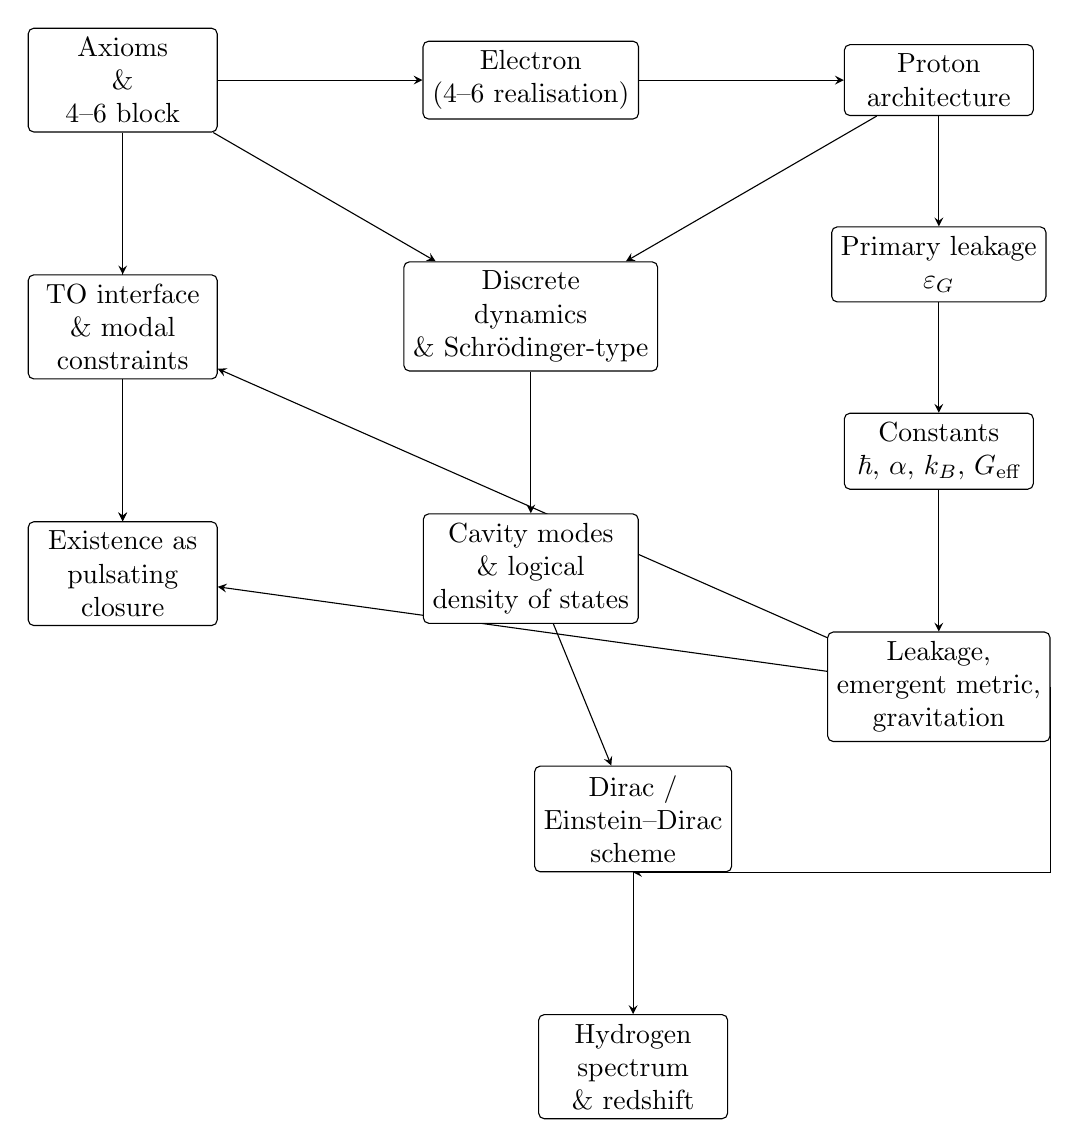
\begin{tikzpicture}[
    node distance=1.6cm,
    box/.style={draw, rectangle, rounded corners=2pt, align=center,
                minimum width=2.4cm, minimum height=0.9cm,
                fill=white},
    >=stealth
  ]
    % Ligne du haut
    \node[box] (axioms) {Axioms \\ \& \\ $4$--$6$ block};
    \node[box, right=2.6cm of axioms] (electron) {Electron \\ $(4$--$6$ realisation)};
    \node[box, right=2.6cm of electron] (proton) {Proton \\ architecture};

    % Colonne proton -> fuite -> constantes -> métrique
    \node[box, below=1.4cm of proton] (eps) {Primary leakage \\ $\varepsilon_G$};
    \node[box, below=1.4cm of eps] (constants) {Constants \\ $\hbar,\, \alpha,\, k_B,\, G_{\text{eff}}$};
    \node[box, below=1.8cm of constants] (metric) {Leakage, \\ emergent metric, \\ gravitation};

    % Colonne centrale gauche : dynamique
    \node[box, below=1.8cm of electron] (dynamics) {Discrete \\ dynamics \\ \& Schr\"odinger-type};

    % Nœud: modes de cavité / densité d'états
    \node[box, below=1.8cm of dynamics] (cavity) {Cavity modes \\ \& logical \\ density of states};

    % Nœud : Dirac / Einstein–Dirac
    \node[box, below=1.8cm of cavity, xshift=1.3cm] (einsteindirac) {Dirac / \\ Einstein--Dirac \\ scheme};

    % Nœud de test phénoménologique
    \node[box, below=1.8cm of einsteindirac] (hydrogen) {Hydrogen \\ spectrum \\ \& redshift};

    % Colonne gauche : interface TO
    \node[box, below=1.8cm of axioms] (TO) {TO interface \\ \& modal \\ constraints};

    % Nœud ontologique : existence as pulsating closure
    \node[box, below=1.8cm of TO] (ontology) {Existence as \\ pulsating \\ closure};

    \begin{pgfonlayer}{background}
      % Chaîne axiomatique
      \draw[->] (axioms) -- (electron);
      \draw[->] (electron) -- (proton);

      % Proton -> fuite -> constantes -> métrique
      \draw[->] (proton) -- (eps);
      \draw[->] (eps) -- (constants);
      \draw[->] (constants) -- (metric);

      % Dynamique
      \draw[->] (axioms) -- (dynamics);
      \draw[->] (proton) -- (dynamics);

      % TO et ontologie
      \draw[->] (axioms) -- (TO);
      \draw[->] (metric) -- (TO);

      % Chaîne dynamique / cavité / Dirac / tests
      \draw[->] (dynamics) -- (cavity);
      \draw[->] (cavity) -- (einsteindirac);
      \draw[->] (metric.east) |- (einsteindirac.south);
      \draw[->] (einsteindirac) -- (hydrogen);

      % Ontologie alimentée par axioms + metric + TO
      \draw[->] (axioms) -- (ontology);
      \draw[->] (metric) -- (ontology);
      \draw[->] (TO) -- (ontology);
    \end{pgfonlayer}

  \end{tikzpicture}
  \caption{Schematic dependency structure within the PDL programme, with the primary
  leakage parameter $\varepsilon_G$ mediating between the proton architecture and the
  constants sector, and feeding into the emergent metric and dynamical layers.}
  \label{fig:pdl_dependency}
\end{figure}


\subsection{Classification scheme}
\label{subsec:classification_scheme}

To systematically assess the internal coherence of the PDL programme and to make explicit the loci at which revisions may be required, we classify each principal component into one of three epistemic categories:
\begin{itemize}[leftmargin=1.5em]
  \item \textbf{Proven structural result:} a proposition established solely on the basis of the axioms and the ensuing combinatorial analysis, without any reliance on phenomenological input.
  \item \textbf{Tightly constrained conjecture:} a proposition that rests on additional, explicitly specified modelling assumptions, yet remains strongly constrained by the axioms, internal consistency conditions, and multiple quantitative correspondences.
  \item \textbf{Empirically calibrated element:} a proposition or construct that involves at least one parameter whose numerical value is fixed by fitting to experimental data, and which has not yet been rigorously derived from the axioms.
\end{itemize}

\subsection{Summary tables}
\label{subsec:summary_tables}

Table~\ref{tab:status} summarises the current epistemic status of selected core components of the PDL framework. This catalogue is intended to be incrementally extended as the research programme progresses and additional theoretical and empirical developments are incorporated.

\setlength{\LTpre}{18pt}
\setlength{\LTpost}{0pt}

\subsection{Global result map: epistemic status}
\label{subsec:global_status}

\begin{longtable}{L{0.8cm}L{2.5cm}L{5cm}L{3.2cm}L{1cm}}
\caption{Schematic status classification for selected structures and results in the current PDL corpus.}
\label{tab:status}\\
\toprule
ID & Domain & Content & Epistemic status & Main sources \\
\midrule
\endfirsthead
\toprule
ID & Domain & Content & Epistemic status & Main sources \\
\midrule
\endhead
\bottomrule
\endfoot

LC1 &
Logical core: axioms and closures &
Relational axioms on finite signed graphs (minimal binary pulsation, triangular coherence, minimal completeness, logical optimisation); definition of closures and coherence measures; identification of the complete signed graph on four vertices and six edges as the first admissible elementary stationary closure. &
Structurally established theorem (within stated axioms). &
\citep{PDL_Main_2026,Minimal_Stationary_Closures_2026,PDL_intro,PDL_position} \\[0.4em]

EL1 &
Electron correspondence &
Minimal correspondence principle identifying the logical $(4,6)$ stationary regime with the electron at rest (Compton oscillation as logical 2‑cycle; $\hbar$ as coherence cost per internal pulsation). &
Tightly constrained physical conjecture. &
\citep{PDL_Main_2026,PDL_intro,PDL_position} \\[0.4em]

PR1 &
Proton architecture &
Hierarchical proton model with three valence cores, relational sea, and active surface; integer tuple $(24,28,930,10087,11017)$ governing internal coherence and surface coupling. &
Tightly constrained structural conjecture (no full uniqueness theorem yet). &
\citep{Combinatorial_Proton_v2_2026,Proton_Local_Uniqueness_2026,PDL_intro,PDL_position} \\[0.4em]

CT1 &
Constants: $\hbar$ as coherence quantum &
Interpretation of $\hbar$ as minimal quantum of action associated with one internal cycle of the $(4,6)$ closure; relation $E=\hbar\omega$ as coherence‑budget statement for the electron at rest. &
Stringently constrained theoretical conjecture. &
\citep{PDL_Main_2026,PDL_intro,PDL_position} \\[0.4em]

CT2 &
Constants: fine‑structure $\alpha$ &
Closed‑form expression for $\alpha_{\PDL}$ in terms of $r_{\mathrm{val}}=930$, the proton–electron mass ratio, and the golden ratio; interpretation as surface‑to‑volume coherence ratio for the proton active surface. &
Tightly constrained conjecture with quantitative agreement at $\mathcal{O}(10^{-4})$. &
\citep{Alpha_PDL_v2_2026,Born_Golden_v2_2026,PDL_intro,PDL_position} \\[0.4em]

CT3 &
Constants: $k_B$ and leakage parameter $\varepsilon$ &
Proposal for $k_B$ in terms of $(4,6)$ structure, proton relational content, dynamical sea fraction, and a minimal leakage parameter $\varepsilon$; interpretation of $k_B$ as granularity scale for thermal coherence in ensembles of closures. &
Stringently constrained conjecture with partial empirical calibration (via $\varepsilon$). &
\citep{PDL_Main_2026,Coherence_Leakage_18_2026,PDL_position} \\[0.4em]

CT4 &
Effective gravitational coupling $G_{\mathrm{eff}}^{\PDL}$ &
Interpretation of macroscopic gravitational coupling as hierarchically filtered coherence leakage from nucleonic structures; discrete exponent $18$ applied to $\varepsilon$ combined with $\hbar$, $c$, and $m_p$ to reproduce the order of magnitude of Newton’s $G$. &
Empirically calibrated construct (functional form fixed; numerical value fitted through $\varepsilon$). &
\citep{Exponent_18_PDL_2026,Coherence_Leakage_18_2026,PDL_Main_2026,PDL_position} \\[0.4em]

CT5 &
Constants: unified leakage bridge between $G$ and $\alpha$ &
Introduction of a primary proton-level leakage parameter $\varepsilon_G$ as the minimal closure defect on the $(r_{\mathrm{val}},R_{\mathrm{sea}})=(930,10087)$ partition. The dimensionless gravitational coupling is represented as $\alpha_G = G m_p^2 / (\hbar c) \simeq \varepsilon_G^{18}$, yielding $\varepsilon_G \approx 0.0073891$, while the electromagnetic valence surplus required by the experimental fine-structure constant, $\Delta r_{\mathrm{val}} \approx 0.0497507$, satisfies the geometric relation $\Delta r_{\mathrm{val}} \approx 3\,\varphi^2\,\varepsilon_G$, thereby locking the gravitational and electromagnetic sectors to a single combinatorial defect in the proton architecture. &
Tightly constrained conjecture (bridge highly sensitive to variations of $G$, $\alpha$, or proton integers). &
\citep{Exponent_18_PDL_2026,Alpha_PDL_v2_2026,Universal_Coherence_Leakage_2026} \\\\[0.4em]


ON1 &
Ontology of pulsating closure &
Ontological reading of PDL as a proposal about persistent existence on finite signed graphs; passage from nothingness to minimal pulsating closure; roles of boundaries, active surfaces, and irreducible leakage as disciplined notions of transcendence; articulation of coexistence topology and multi‑observer stabilisation, with careful linkage to the technical corpus. &
Conceptual framework disciplined by technical results (philosophically oriented but structurally anchored). &
\citep{ExistencePulsatingClosure2026,PDL_Main_2026,PDL_position,PDL_TO_dialogue} \\[0.4em]

DY1 &
Graph dynamics and emergent Schr\"odinger‑type equations &
Families of local sign‑update rules on signed graphs aimed at implementing coherence‑optimising dynamics; preliminary sketches of how Schr\"odinger‑type equations may emerge in coarse‑grained limits; benchmark analyses of hydrogenic spectra using PDL‑derived $\alpha$ and proton parameters. &
Open dynamical programme with partial consistency evidence. &
\citep{Effective_Fields_PDL_2026,Schrodinger_Sketch_v2_2026,Schrodinger_PDL_v2_2026,PDL_position} \\[0.4em]

DY2 &
Cavity modes and logical density of states &
Construction of a three‑dimensional PDL cavity as a finite signed graph; definition of a photon‑like logical excitation indexed by $(n_x,n_y,n_z)$; identification of low‑leakage periodic modes with minimal period $N(n_x,n_y,n_z)=4(n_x+n_y+n_z)$ for a broad family; and derivation of an effective logical density of states scaling $\rho(\nu)\propto \nu^2$ in three dimensions, mirroring continuum cavity mode counting. &
Tightly constrained dynamical conjecture (fully explicit but currently supported by numerical evidence on specific graphs). &
\citep{PDLCavityModes2026,Effective_Fields_PDL_2026} \\[0.4em]

TI1 &
Interface with Theory of Objectivity (TO) &
Modal dialogue between PDL and TO; mapping of PDL closures to TO’s objects and boundaries; analysis of multi‑observer stabilisation and the role of a transcendent substrate supporting incomplete closures. &
Conceptual synthesis and compatibility analysis (framework‑level proposal). &
\citep{PDL_TO_dialogue,PDL_position,ExistencePulsatingClosure2026} \\[0.4em]

\end{longtable}

\subsection{Dependency diagram (conceptual)}

\begin{figure}[H]
  \centering
  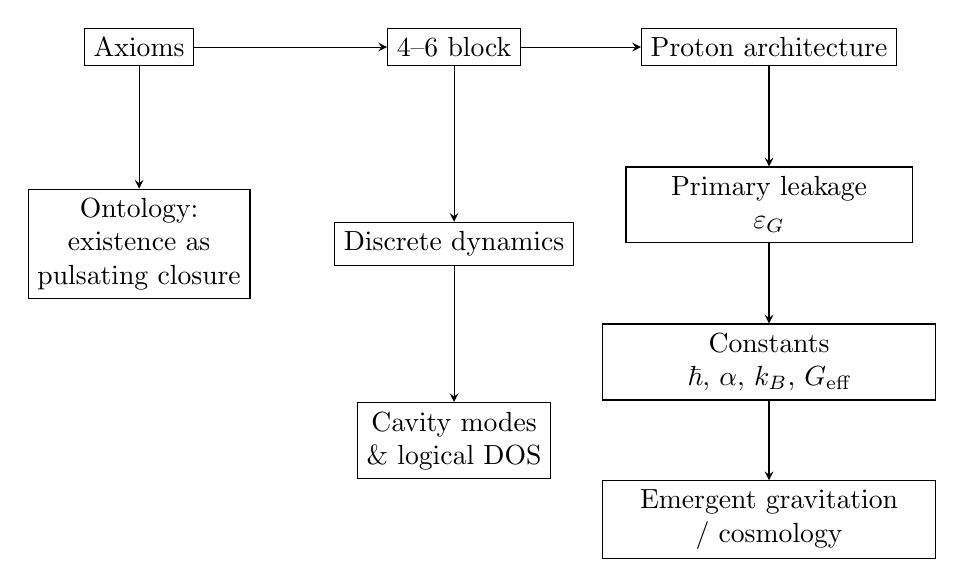
\begin{tikzpicture}[node distance=2cm,>=stealth,->]
    % Ligne de base : axioms -> 4-6 -> proton -> epsilon_G -> constants -> gravitation
    \node (axioms)   [draw, rectangle, fill=white] {Axioms};
    \node (fourSix)  [draw, rectangle, fill=white, right of=axioms, xshift=2cm] {4--6 block};
    \node (proton)   [draw, rectangle, fill=white, right of=fourSix, xshift=2cm] {Proton architecture};

    \node (eps)      [draw, rectangle, fill=white, below of=proton, text width=3.4cm, align=center]
                     {Primary leakage \\ $\varepsilon_G$};
    \node (constants)[draw, rectangle, fill=white, below of=eps, text width=4cm, align=center]
                     {Constants \\ $\hbar,\,\alpha,\,k_B,\,G_{\text{eff}}$};
    \node (grav)     [draw, rectangle, fill=white, below of=constants, text width=4cm, align=center]
                     {Emergent gravitation \\ / cosmology};

    % Branche ontologique
    \node (ontology) [draw, rectangle, fill=white, below of=axioms, yshift=-0.5cm, align=center]
                     {Ontology: \\ existence as \\ pulsating closure};

    % Branche dynamique / cavité
    \node (dynamics) [draw, rectangle, fill=white, below of=fourSix, yshift=-0.5cm]
                     {Discrete dynamics};
    \node (cavity)   [draw, rectangle, fill=white, below of=dynamics, yshift=-0.5cm, align=center]
                     {Cavity modes \\ \& logical DOS};

    % Flèches
    \draw (axioms) -- (fourSix);
    \draw (fourSix) -- (proton);
    \draw (proton) -- (eps);
    \draw (eps) -- (constants);
    \draw (constants) -- (grav);

    \draw (axioms) -- (ontology);
    \draw (fourSix) -- (dynamics);
    \draw (dynamics) -- (cavity);
  \end{tikzpicture}
  \caption{Conceptual dependency chain within PDL, with the primary leakage parameter
  $\varepsilon_G$ mediating between the proton architecture and the constants sector, together
  with the ontological reading of pulsating closure and the cavity-mode sector with logical
  density of states.}
  \label{fig:dependency}
\end{figure}



\section{Roadmap and Future Work}
\label{sec:roadmap}

\subsection{Foundational and combinatorial tasks}
\label{subsec:roadmap_foundational}

Several foundational combinatorial problems are pivotal for the further development of the PDL programme. The first concerns the uniqueness of the minimal $4$–$6$ block. Providing a rigorous proof or disproof that no smaller or alternative configuration satisfies the axioms with comparable optimality would determine whether the $4$–$6$ regime constitutes a strictly necessary primitive or merely one admissible element within a broader class of allowable structures \citep{PDL_Main_2026,PDL_position}. 

A second major objective is the exhaustive classification of admissible proton architectures in a neighbourhood of the integer tuple $(24,28,930,10087,11017)$. The aim is to ascertain whether the currently favoured proton model is uniquely determined (up to isomorphism) by the underlying optimisation constraints, or whether there exists a nontrivial family of degenerate alternatives that remain consistent with the same criteria \citep{Combinatorial_Proton_v2_2026,PDL_position}. 

A third foundational goal is to obtain a purely combinatorial derivation of the leakage parameter $\varepsilon$ and the exponent $18$ from intrinsic graph-theoretic invariants of hierarchical closures. Achieving this would obviate the current dependence on calibration against the empirical value of $G$, thereby promoting gravitation from a partially fitted phenomenon to a fully predicted emergent coupling \citep{Exponent_18_PDL_2026,Coherence_Leakage_18_2026,PDL_position}.
\paragraph{(R\_Leakage) Primary leakage parameter and $G$--$\alpha$ bridge.}

Beyond the generic notion of logical leakage $\varepsilon$ introduced in earlier work, the recent analysis of universal coherence leakage identifies a primary, proton-level leakage parameter $\varepsilon_G$ as the central quantity of interest.\citep{Universal_Coherence_Leakage_2026}
This parameter is inferred from the dimensionless gravitational coupling
\[
\alpha_G = \frac{G m_p^2}{\hbar c} \simeq \varepsilon_G^{18},
\]
together with the proton partition
\[
(r_{\mathrm{val}}, R_{\mathrm{sea}}) = (930, 10087),
\]
and is numerically constrained to
\[
\varepsilon_G \approx 0.0073891.\citep{Coherence_Leakage_18_2026,Universal_Coherence_Leakage_2026}
\]
Independently, the structural representation of the fine-structure constant and the active-surface geometry
\[
R_{\mathrm{surf}} = \varphi\,\frac{r_{\mathrm{val}}}{3}
\]
imply an electromagnetic valence surplus
\[
\Delta r_{\mathrm{val}} \approx 0.0497507
\]
required to reproduce the empirical value $\alpha_{\exp}$.\citep{Alpha_PDL_v2_2026}
The Universal Coherence Leakage analysis establishes that these two quantities are connected via a geometric relation of the form
\[
\Delta r_{\mathrm{val}} \approx 3\,\varphi^2\,\varepsilon_G,
\]
indicating that the gravitational and electromagnetic sectors are jointly constrained by a single combinatorial defect in the internal proton architecture.

The research agenda for this sector can be structured into three tightly interrelated objectives:
\begin{enumerate}[label=(\roman*), leftmargin=*]
  \item \emph{Derivation of $\varepsilon_G$ from first principles.}  Replace the current determination of $\varepsilon_G$ from the empirical value of $G$ with an explicit graph-theoretic computation of the minimal frustration density on admissible proton graphs satisfying $(r_{\mathrm{val}},R_{\mathrm{sea}})=(930,10087)$. This would eliminate the remaining phenomenological calibration in the leakage sector and yield a fully model-intrinsic definition of $\varepsilon_G$.
  \item \emph{Uniqueness and robustness of the $G$--$\alpha$ bridge.}  Delineate the admissible range of combinatorial parameters within which the relation $\Delta r_{\mathrm{val}} \approx 3\,\varphi^2\,\varepsilon_G$ remains valid under controlled perturbations of the proton integer tuple $(24,28,930,10087,11017)$. In addition, investigate whether alternative PDL-compatible architectures exist that simultaneously reproduce $G$ and $\alpha$ while violating this bridge relation, thereby systematically probing the uniqueness and structural stability of the proposed $G$--$\alpha$ correspondence.
  \item \emph{Extension to additional constants and cosmological observables.}  Investigate whether the same primary leakage parameter $\varepsilon_G$ can be utilized, without the introduction of additional free parameters, in refined constructions for $k_B$, $G_{\mathrm{eff}}^{\PDL}$, and coherence-induced cosmological contributions. Evaluate the extent to which these extended schemes can be confronted with, and jointly constrained by, current and forthcoming observational data.
\end{enumerate}
Within the global result map presented in Section~\ref{sec:global_map}, these issues are represented by the status of the unified leakage bridge (entry CT5 in Table~\ref{tab:status}) and by the newly introduced document D20. Together, these elements characterize the transition from a phenomenologically tuned leakage parameter to a structurally constrained coupling construct that mediates between microphysical and macrophysical descriptions.


\subsection{Dynamical and phenomenological extensions}
\label{subsec:roadmap_dynamical}

On the dynamical side, a primary objective is to specify and rigorously analyse a canonical class of graph-evolution rules that satisfy the PDL axioms, implement energy as a coherence cost, and recover Schr\"odinger-type evolution equations in appropriate coarse-grained limits \citep{Coherence_Leakage_18_2026,Coherence_Leakage_18_2026}. This requires elucidating the mechanisms by which probability amplitudes, interference patterns, and measurement-like phenomena arise from discrete coherence flows on signed graphs. At the phenomenological level, the existing benchmarks based on the hydrogen atom must be extended to more complex systems, including alternative nuclei, hydrogen-like ions, simple multi-electron atoms, and condensed-matter configurations \citep{PDL_Main_2026,Schrodinger_Sketch_v2_2026}. Such extensions will facilitate a systematic investigation of the scaling behaviour of coherence-ratio representations and furnish a stringent test of whether the PDL architecture remains self-consistent as structural and dynamical complexity increase \cite{PDL_position}.

\subsection{Interface and comparison with other frameworks}
\label{subsec:roadmap_interface}

A further line of investigation is concerned with the systematic comparison of PDL with other foundational frameworks. This research programme encompasses a confrontation of the discrete coherence structures underlying PDL with quantum field theory and quantum chromodynamics—particularly in relation to proton structure and the decomposition of proton mass—as well as with quantum-information–theoretic reconstructions of quantum theory and with discrete or holographic approaches, including causal set theory, loop-based models, and tensor network formalisms \citep{PDL_intro,PDL_position}. The overarching aim is to characterise the domains in which PDL reproduces established results, generates genuinely novel theoretical insights, or can be subjected to stringent empirical or purely theoretical tests capable of yielding decisive falsification. In parallel, a more intensive engagement with the Theory of Objectivity and related modal–axiomatic programmes is anticipated to refine the ontological interpretation of PDL, in particular regarding the nature of boundaries, the stabilisation of structures across multiple observers, and the status of the leakage parameter as a candidate for a transcendent substrate \citep{PDL_TO_dialogue,PDL_position}.

\subsection{Planned updates of this mapping document}
\label{subsec:roadmap_mapping}

This mapping document is intended as a dynamic, continuously maintained overview of the PDL programme. It will be updated whenever significant milestones are attained, such as the proof of a uniqueness theorem for the $4$--$6$ block, a combinatorial derivation of $\varepsilon$, a mathematically rigorous account of emergent Schr\"odinger dynamics, or substantial revisions of the proton architecture \citep{PDL_position}. Subsequent updates will refine the global result map, introduce or modify entries in the document index, and adjust the dependency diagrams so as to represent faithfully the evolving internal structure of the programme. Negative results and counterexamples will be recorded explicitly, thereby ensuring that the mapping continues to function as a transparent structural framework for assessing both the achievements and the limitations of the PDL approach \citep{PDL_position}.

\newpage

\appendix

\section{Document Index and Cross-References}
\label{app:doc_index}

Table~\ref{tab:doc_index} provides an overview of the principal PDL documents, the internal identifiers assigned to them within this mapping (D1, D2, \dots), and a concise description of the sections of the present study in which each document is predominantly utilised.

\setlength{\LTpre}{18pt}
\setlength{\LTpost}{0pt}

\begin{longtable}{@{}p{0.9cm}L{5cm}L{5cm}p{4.4cm}@{}}
  \caption{Index of PDL documents and their role in this mapping.}
  \label{tab:doc_index}\\

  \toprule
  Label & Document & Main thematic domain & Sections of this mapping \\
  \midrule
  \endfirsthead

  \toprule
  Label & Document & Main thematic domain & Sections of this mapping \\
  \midrule
  \endhead

  \bottomrule
  \endfoot

  D1 &
  The Emergence of Physical Reality within the Framework of the Projective Dynamic Logo (PDL) &
  Core axioms, $4$--$6$ block, proton architecture, constants, gravitation, cosmology &
  \ref{sec:logical_core}, \ref{sec:four_six_electron}, \ref{sec:proton_architecture}, \ref{sec:constants}, \ref{sec:topology_metric} \\[0.4em]

  D2 &
  Introduction to the Projective Dynamic Logo (PDL) &
  High-level conceptual overview and summary of key structures and constants &
  \ref{sec:overview}, \ref{subsec:core_question}, \ref{sec:constants}, \ref{sec:roadmap} \\[0.4em]

  D3 &
  Projective Dynamic Logo as a Foundational Research Programme (Position Paper) &
  Status, epistemic classification, open problems, TO dialogue, global mapping of results &
  \ref{sec:overview}, \ref{sec:global_map}, \ref{sec:TO_interface}, \ref{sec:roadmap} \\[0.4em]

  D4 &
  On the Combinatorial Selection of the Proton Architecture in PDL (v2) &
  Detailed proton integers, optimisation constraints, alternative candidates, updated selection functional &
  \ref{sec:proton_architecture}, \ref{subsec:roadmap_foundational} \\[0.4em]

  D5 &
  A Structural Derivation of the Fine-Structure Constant from the Projective Dynamic Logo (PDL) (v2) &
  Derivation and numerical assessment of the PDL expression for $\alpha$, including post-TO refinements &
  \ref{sec:constants}, \ref{subsec:constants_table}, \ref{sec:global_map} \\[0.4em]

  D6 &
  Relational Emergence of Born's Rule and a Golden-Ratio Active Surface in PDL (v2) &
  Born's rule for spin-$\tfrac{1}{2}$, golden-ratio active surface, refined link between surface partition and $\alpha$ &
  \ref{sec:logical_core}, \ref{sec:constants}, \ref{sec:global_map} \\[0.4em]

  D7 &
  From Discrete Coherence Flux to Effective Fields: A Structured Programme within the PDL Framework &
  Discrete Gauss–Faraday structure, effective fields, Coulomb profiles, link to Schr\"odinger-type dynamics &
  \ref{sec:dynamics}, \ref{sec:topology_metric}, \ref{sec:global_map} \\[0.4em]

  D8 &
  A Minimal Relational Sketch for the Emergence of the Golden Ratio in PDL &
  Core–surface partition of the proton, emergence of the golden ratio, constraints on active surface &
  \ref{sec:proton_architecture}, \ref{sec:constants} \\[0.4em]

  D9 &
  Hierarchical Filtering of Coherence Leakage and Justification of the Exponent 18 in PDL &
  Original formulation of leakage filters and exponent $18$ as total number of hierarchical filters &
  \ref{sec:topology_metric}, \ref{subsec:roadmap_foundational} \\[0.4em]

  D10 &
  Logical Leakage as Self-Maintained Probability: A Topological Reformulation in the Projective Dynamic Logo Framework &
  Coexistence topology, coherence-cost pseudo-metric, probabilistic reinterpretation of leakage &
  \ref{sec:topology_metric}, \ref{sec:dynamics}, \ref{sec:global_map} \\[0.4em]

  D11 &
  Compatibility of the Schr\"odinger Framework with the Projective Dynamic Logo (PDL) (v2) &
  Effective insertion of PDL-derived $\alpha$ and proton structure into hydrogenic Schr\"odinger equation, updated numerical checks &
  \ref{sec:dynamics}, \ref{sec:global_map} \\[0.4em]

  D12 &
  Towards a Schr\"odinger--Type Dynamics from the Projective Dynamic Logo (PDL): A Relational Sketch Linking Coherence Cycles, Active Surfaces, and Effective Potentials (v2) &
  Toy models and preliminary derivations of Schr\"odinger-like dynamics from graph evolution, refined consistency conditions &
  \ref{sec:dynamics}, \ref{subsec:roadmap_dynamical} \\[0.4em]

  D13 &
  A Modal Dialogue between the Projective Dynamic Logo (PDL) and the Theory of Objectivity (TO) &
  Comparison with TO's Absolute Truths, boundary and multi-observer issues, transcendent substrate &
  \ref{sec:TO_interface}, \ref{subsec:roadmap_interface} \\[0.4em]

  D14 &
  Towards an Einstein--Dirac Unification from the Projective Dynamic Logo Framework &
  Einstein–Dirac extension, Dirac spinors on $(4,6)$ closures, coupling to emergent metric, preliminary consistency checks &
  \ref{sec:dynamics}, \ref{sec:topology_metric}, \ref{subsec:roadmap_dynamical} \\[0.4em]

  D15 &
  Minimal Stationary Closures in the Projective Dynamic Logo Framework: Necessity of the (4,6) Block &
  Detailed analysis of minimal stationary closures, non-existence for $n \leq 3$, necessity and quasi-uniqueness of the $(4,6)$ block &
  \ref{sec:logical_core}, \ref{subsec:4_6_block}, \ref{sec:global_map} \\[0.4em]

  D16 &
  On the Combinatorial Selection and Local Uniqueness of the Proton Architecture in the PDL Framework &
  Refined combinatorial analysis of proton configurations, definition of selection functional, local uniqueness conjecture &
  \ref{sec:proton_architecture}, \ref{subsec:roadmap_foundational} \\[0.4em]

  D17 &
  Coherence Leakage, Hierarchical Filtering, and the Exponent 18 in the Projective Dynamic Logo Framework &
  Refined treatment of coherence leakage, intrinsic $\varepsilon$ on proton graphs, organisation of 18 filters, and an effective coupling ansatz for $G_{\mathrm{eff}}^{\PDL}$, which in the present mapping is instantiated with the primary proton-level leakage parameter $\varepsilon_G$ inferred from the dimensionless gravitational coupling.
 &
  \ref{sec:topology_metric}, \ref{sec:global_map}, \ref{subsec:roadmap_foundational} \\[0.4em] 

  D18 & 
  Existence as Pulsating Closure: An Ontological Meditation on the PDL Framework & Ontological and philosophical analysis of PDL as a proposal about persistent existence on finite signed graphs; passage from nothingness to minimal pulsating closure; roles of boundaries, active surfaces, and irreducible leakage as disciplined notions of transcendence; articulation of coexistence topology and multi-observer stabilisation, explicitly tied back to the technical corpus. & 
  \ref{sec:overview}, \ref{sec:topology_metric}, \ref{sec:roadmap} \\[0.4em] 
  
  D19 & 
  Discrete Cavity Modes and Logical Density of States in the PDL Framework & Construction of a three-dimensional PDL cavity as a finite signed graph; definition of a photon-like logical excitation indexed by $(n_x,n_y,n_z)$; identification of low-leakage periodic modes with minimal period $N(n_x,n_y,n_z)=4(n_x+n_y+n_z)$; and derivation of an effective logical density of states scaling $\rho(\nu)\propto \nu^2$ in three dimensions, used in the discussion of dynamical structures. & 
  \ref{sec:dynamics}, \ref{subsec:cavity_modes} \\[0.4em]

  D20 &
  Universal Coherence Leakage: Bridging Gravitational and Fine-Structure Constants through Discrete Relational Closures &
  Primary proton-level leakage parameter $\varepsilon_G$ on the $(r_{\mathrm{val}},R_{\mathrm{sea}})=(930,10087)$ partition; exponent-18 hierarchical filtering $\alpha_G \simeq \varepsilon_G^{18}$; and geometric bridge to the electromagnetic sector via the valence surplus $\Delta r_{\mathrm{val}} \approx 3\,\varphi^2 \varepsilon_G$ that locks $G$ and $\alpha$ to a single combinatorial defect in the proton architecture. &
  \ref{sec:constants}, \ref{sec:topology_metric}, \ref{sec:global_map} \\\\[0.4em]

\end{longtable}

\section{Glossary of Selected Terms}
\label{app:glossary}

\begin{description}[style=nextline,leftmargin=1.5cm]
  \item[Closure] A finite signed graph that realises a self-sustaining regime of
  coherence under the PDL axioms, exhibiting minimal or otherwise controlled
  leakage.

  \item[Logical stationary regime] A configuration whose internal sign
  pattern sustains a non-trivial cyclic evolution (typically a 2-cycle)
  that preserves triangular coherence and does not rely on external input.

  \item[Coherence cost] A quantitative measure of the relational “effort”
  necessary to maintain a given closure; in physical instantiations, this
  quantity can be identified with energy via relations such as \(E = \hbar \omega\).

  \item[Active surface] The subset of relations within a composite structure
  (for example, the proton) that actually participate in coherent coupling to
  external closures, in contrast to relations that are dedicated exclusively
  to internal stabilisation.

  \item[Leakage] The minimal, irreducible defect of closure in hierarchical
  structures, parameterised by \(\varepsilon\); this is interpreted both as
  a source of effective probabilistic behaviour and as the origin of emergent
  gravitational coupling.

  \item[Coexistence topology] The topology on the space of closures induced by
  their mutual compatibility; two closures are considered “close” if they can
  be jointly embedded with a low additional coherence cost.

  \item[Coherence-cost pseudo-metric] A distance-like function on the space of
  closures, which measures the extra coherence expenditure required to render
  them coexistent within a common environment; this provides the discrete
  substrate for an emergent metric structure.

\end{description}

\section{Glossary of Key Terms}
\label{app:key_glossary}

\begin{description}[style=nextline,leftmargin=1.5cm]

\item[Closure]
A finite signed graph that realises a self-sustaining regime of coherence under the PDL axioms: all required triangular constraints are satisfied (or minimally violated in a controlled way), and the structure is logically autonomous (no dependence on an unspecified background). 

\item[Logical stationary regime]
A dynamical regime in which the internal sign configuration of a closure undergoes a non-trivial cyclic evolution (typically a logical 2-cycle) that preserves triangular coherence and can be maintained indefinitely without external input; the $(4,6)$ block is the prototype example.

\item[Coherence cost]
A quantitative measure of the relational “effort” required to maintain a given closure or stationary regime. In physical interpretations, this cost is identified with energy, and relations such as \(E = \hbar \omega\) express the coherence budget needed per internal pulsation cycle.

\item[Active surface]
The finite set of relations through which a composite structure (notably the proton) is available for coherent coupling to external closures. The active surface mediates interactions (e.g. electron–proton binding) and plays a central role in surface-to-volume coherence ratios used to reinterpret constants such as the fine-structure constant.

\item[Leakage]
The irreducible fraction of violated coherence constraints in an optimised composite closure, quantified by a parameter \(\varepsilon\). Leakage encodes a minimal, structured export of coherence constraints into the surrounding network and underlies both probabilistic behaviour and the emergence of effective gravitational couplings.

\item[Cavity mode]
A low-leakage, strictly periodic excitation of a finite PDL cavity graph, typically indexed by integer triples \((n_x,n_y,n_z)\), whose minimal period defines a logical wavelength and frequency. The counting of such modes yields an effective three-dimensional logical density of states with \(\rho(\nu)\propto \nu^2\).

\end{description}


\bibliographystyle{plain}
\bibliography{references}

\end{document}
